%%%%%%%%%%%%%%%%%%%%%%%%%%%%%%%%%%%%%%%%%
% Journal Article
% LaTeX Template
% Version 2.0 (February 7, 2023)
%
% This template originates from:
% https://www.LaTeXTemplates.com
%
% Author:
% Vel (vel@latextemplates.com)
%
% License:
% CC BY-NC-SA 4.0 (https://creativecommons.org/licenses/by-nc-sa/4.0/)
%
% NOTE: The bibliography needs to be compiled using the biber engine.
%
%%%%%%%%%%%%%%%%%%%%%%%%%%%%%%%%%%%%%%%%%

%----------------------------------------------------------------------------------------
%	PACKAGES AND OTHER DOCUMENT CONFIGURATIONS
%----------------------------------------------------------------------------------------

\documentclass[
	a4paper, % Paper size, use either a4paper or letterpaper
	10pt, % Default font size, can also use 11pt or 12pt, although this is not recommended
	unnumberedsections, % Comment to enable section numbering
	twoside, % Two side traditional mode where headers and footers change between odd and even pages, comment this option to make them fixed
]{LTJournalArticle}
\usepackage{biblatex}
\usepackage{authblk} 
\usepackage{subfigure}
\usepackage{lipsum}  
\usepackage{subcaption}
\usepackage{caption}
\usepackage{tabularx}
\usepackage{amsmath,amsfonts,amssymb}
\captionsetup{width=.45\textwidth}
\addbibresource{biblio.bib} % BibLaTeX bibliography file

\runninghead{Deep learning project report} % A shortened article title to appear in the running head, leave this command empty for no running head

% \footertext{\textit{Journal} (Year) DOI/ISBN} % Text to appear in the footer, leave this command empty for no footer text

\setcounter{page}{1} % The page number of the first page, set this to a higher number if the article is to be part of an issue or larger work

%----------------------------------------------------------------------------------------
%	TITLE SECTION
%----------------------------------------------------------------------------------------

\title{Projet de deep learning\\ \LARGE Estimation des distances entre les individus dans une image.} % Article title with subtitle


% Authors are listed in a comma-separated list with superscript numbers indicating affiliations
% \thanks{} is used for any text that should be placed in a footnote on the first page, such as the corresponding author's email, journal acceptance dates, a copyright/license notice, keywords, etc
\author{%
    Ilann Amiaud--Plachy\textsuperscript{1},
    Gaétan Jacquemin\textsuperscript{1}
}

\date{\footnotesize\textsuperscript{\textbf{1}}CentraleSupélec, Paris-Saclay University}

% Affiliations are output in the \date{} command
% \date{\footnotesize\textsuperscript{\textbf{1}}Immersive Audio, L-Acoustics UK Ltd\\ \textsuperscript{\textbf{2}}MSc Student in Information and Comms. Eng., CentraleSupélec, Paris-Saclay University}

% Full-width abstract
\renewcommand{\maketitlehookd}{%
	\begin{abstract}
		Nous nous sommes intéressés à l’estimation des distances entre les personnes dans une foule à partir d’une image monoculaire. Notre solution se concentre spécifiquement sur les distances entre les têtes, qui sont les seuls éléments clairement détectables dans ce contexte. Face à l’absence de modèles directement adaptés à cette tâche dans l’état de l’art, nous avons développé une approche hybride. Celle-ci repose sur deux modèles : un modèle de détection d’objets, affiné sur un jeu de données adapté pour identifier les têtes, et un modèle d’estimation de carte de profondeur. En combinant ces deux estimations, nous avons modélisé le fonctionnement de la caméra et utilisé les lois de l’optique géométrique pour, d’une part, corriger la carte de profondeur estimée, et d’autre part, calculer les distances entre les têtes. Nos résultats sont qualitativement prometteurs, mais une évaluation quantitative reste nécessaire pour les valider pleinement.
	\end{abstract}
}

%----------------------------------------------------------------------------------------
%----------------------------------------------------------------------------------------

\begin{document}

    \maketitle % Output the title section

    %----------------------------------------------------------------------------------------
    %	ARTICLE CONTENTS
    %----------------------------------------------------------------------------------------

    \section{Introduction}

         


\lipsum[1-2]

    \section{Détection des têtes}

        
\subsection{Etat de l'art des modèles}

Vous pourrez trouver un recensement des références de modèles et de dataset (paper et code) sur ce répertoire github \cite{state_of_the_art_crowd_counting}. Beaucoup de modèles existent déjà pour la détection des têtes, mais pour ce projet et pour apprentissage nous avons décidé d'utiliser YOLOv11 \cite{khanam2024yolov11overviewkeyarchitectural}, avec un finetuning sur notre dataset d'images.

ILANN BLABLABLA

\subsection{Datasets}

Il existe plusieurs datasets pour la détectiond des têtes et avec l'utilisation grandissante des cameras comme moyens de surveillance, ils se sont multipliés et sont de plus en plus gros. On dispose donc de beaucoup de matériel pour notre entrainement et évaluation, certains articles \cite{state_of_the_art_datasets} proposent des benchmarks pour les datasets les plus utilisés.

Pour notre utilisation, nous cherchons des datasets avec un nombre de personne supérieur à 100, car nous souhaitons nous intérresser spécifiquement aux foules denses. Pour cela nous avons sélectionnés les datasets JHU-Crowd++ \cite{sindagi2020jhu-crowd++} (le seul utilisé dans ce projet en réalité) qui présente 4372 avec en moyenne 346 personnes et jusque 25,791.
Nous avons selectionné 2 autres datasets semblables que nous n'avons pas utilisé dans ce projet, le NWPU-Crowd \cite{gao2020nwpu} avec 5,109 images d'en moyenne 418 personnes, et le UCF-QNRF \cite{idress2018ucfqnrf} avec 1,535 images d'en moyenne 815 personnes.

\subsection{Finetuning}

ILANN BLABLABLA

    \section{Estimation monoculaire de la profondeur}

        
L'estimation monoculaire de la profondeur est un problème qui consiste à déterminer la distance à la caméra de chaques pixels d'une image en se basant uniquement sur l'image elle-même.

C'est un problème complexe d'actualité avec beaucoup d'application, comme la segmentation des objets ou la reconstruction 3D (pour le cinéma ou pour la modélisation). L'estimation de la profondeur est certe réalisable avec des technologies de prise de vue particulières (comme la stéréovision), mais avec une estimation monculaire transforme n'importe quelle caméra en un capteur de profondeur.

\subsection{Etat de l'art}

Comme expliqué précedemment, du fait de ses applications industrielles direct, ce problème est déjà largement adressé et des modèles de deep learning sont déjà incroyablement performants. Pour ceux proche de notre application on retiendra \textit{DepthAnythingv2} \cite{depthanythingv2}, \textit{Monodepth2} \cite{MonoDepth2}, ou encore \textit{Depth Pro} \cite{depthpro} de apple qui vient tout juste de sortir.

On peut citer aussi \textit{DenseDepth} \cite{DenseDepth} pour de la prédiction sur des images 360°.

\subsection{Choix \& résultat}

Pour la réalisation de ce projet et après les avoir essayé notre choix s'est porté sur \textit{DepthAnythingv2} pour plusieurs raisons. En premier lieu, il faut comprendre que la plupart des modèles d'estimation monoculaire marchent bien sur des champs proches, mais ont tendance à être limité sur des champs lointains. Or ce qui nous interresse, comme nous utilisons des images extérieures à ciel ouvert (souvent), il s'agit souvent de champs lointains et extérieur, ce qui ne correspond pas aux datasets d'entrainement de ces modèles. 

Or justement \textit{depthanythingv2} propose une version "outdoor" et en système métrique, ce qui convient précisément à notre application, notre choix s'est donc porté sur ce modèle et nous avons obtenu des résultats satisfaisants.

EXEMPLE DE RESULTAT





    \section{Correction de la carte de profondeur}

        
Le problème est que le résultat est satisfaisant visuellement, mais après exploitation (expliquée ci-dessous) on s'est rendu compte que l'on avait pas des résultats très cohérent suivant si on se trouvait dans un champs proche ou lointain. par exemple une distance entre têtes dans un champs lointain parraissait cohérente tandis que une distance entre têtes dans un champs proche était beaucoup trop grande. On a donc décidé de corriger cette carte de profondeur en lui appliquant une transformation.

Pour se faire, et comme c'est les têtes qui nous intéressent, on s'est appuyé sur elles pour corriger la carte de profondeurs. En effet, avec un peut de recherche dans la litérature on comprend que les têtes font sensiblement toutes la même taille, en tout cas qu'il y a une faible variance dans la population.

Et justement grâce à notre modèle finetuné de \textit{Yolov11}, pour les têtes detectés on a une boite englobante de la tête qui est assez précise. Par ailleur,  on a la relation suivante 

\begin{figure}
    \centering
    % \includegraphics[width=0.8\textwidth]{depth_correction_formula.png}
    \caption{Schémas de l'optique d'un appareil photo.}
    \label{fig:depth_correction_formula}
\end{figure}

\begin{equation} \label{eq:camera_relation}
    \frac{\text{width (pxl)}}{\text{focale (pxl)}} = \frac{\text{width (m)}}{\text{depth (m)}}
\end{equation}


comme notre focale d'appareil est une constante, alors le produit $ \text{width} \times \text{depth} $  est proportionnel à la taille de la tête et doit donc être également répartie et ne pas dépendre de la prodonfeur, hors ce n'est pas ce que l'on observe, on voit nettement une correlation. 

\begin{figure}
    \centering
    % 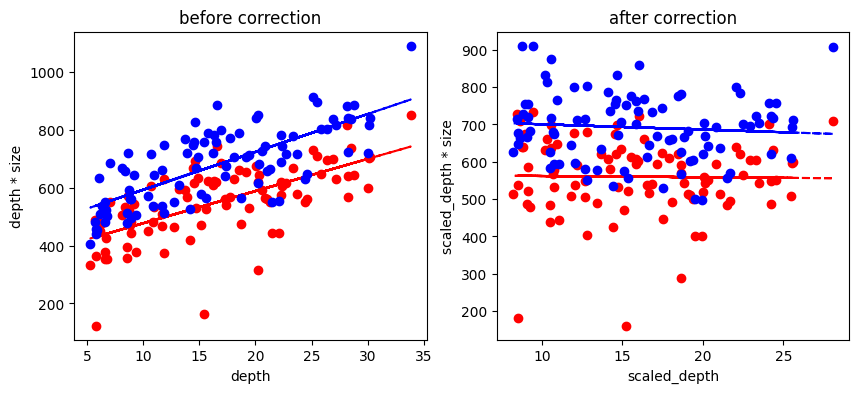
\includegraphics[width=0.8\textwidth]{depth_correction.png}
    \caption{(à gauche) avant la correction, on voit la corrélation. (à droite) la correction annule la correlation. }
    \label{fig:depth_correction}
\end{figure}

On effectue donc une régression linéaire pour déterminer une correctione linéaire à la carte de profondeur qui permet d'annuler la correlation entre le produit expliqué et la taille des têtes.



    \section{Estimation de la focale}

        

On détermine aussi la focale grâce à la taille des têtes. En effet, grâce à la relation \ref{eq:camera-relation} On estime une valeur de la focale pour chaques tête détecté, en supposant que une tête doit avoir des mensurations constantes(pour la largeur et pour la hauteur), on prend les mensurations suivantes (tiré d'études statistiques):

\begin{itemize}
    \item hauteur : 22cm
    \item largeur : 19cm
\end{itemize}

Finalement, on prend comme focale le maximum de la distribution des focales estimées pour chaques têtes (voir Figure \ref{fig:focal-estimation}). On se base au finale seulement sur les focales estimés à partir de la hauteur de la tête après avoir empiriquement constaté une meilleur constance de la hauteur que de la largeur.

\begin{figure}[h!]
    \centering
    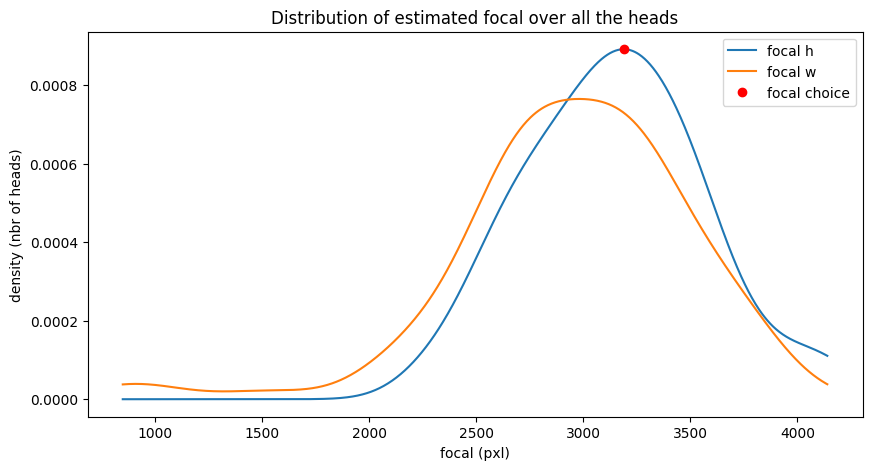
\includegraphics[width=0.45\textwidth]{images/focal_choice.png}
    \caption{Distribution des focales estimées pour chaque têtes, et choix de la valeur estimé de la focale (en pixels).}
    \label{fig:focal-estimation}
\end{figure}

Cette focale est très importante puisque c'est elle qui nous permet de calculer la ditance sur l'axe X en fonction de la profondeur (toujours grâce à la relationn \ref{eq:camera-relation}).

    \section{Estimation des distances}

        

Pour l'estimation des distance on doit décomposer l'espace en plusieurs dimensions. Pour simplifier on va diviser l'espace en 2 dimensions.

Pour 2 têtes, On prend comme référence le plan qui passe par ces 2 têtes et dont une des 2 dimensions est parrallêle au sol (donc au bord inférieur de l'image). Ainsi on a les 2 dimensions:

\begin{itemize}
    \item la dimension X est la dimension parrallêle au bord inférieur de l'image
    \item la dimension Y est celle perpendiculaire à celle-ci, mais qui suit le plan passant par les 2 têtes.
\end{itemize}


Ainsi, en obtenant la projection de lu vecteur disctantce sur ces 2 dimensions, on calcul la distance totale avec le théorème de pythagore.

Par ailleurs on notera : $(x_1, y_1)$ et $(x_2, y_2) $les coordonnées des 2 têtes (en pixel), $(d_1,d_2)$ leur profondeur respective (en mêtre) et $(dX, dY)$ le vecteur distance entre les 2 têtes (en mêtres). Et $f$ la focale de la caméra (en pixel).

\subsection{distance sur l'axe Y}

Pour calculer la distance sur l'axe y, qui est en fait la différence de profondeur corrigé pour prendre en compte la position relative des personnes, on utilise le théorème d'alkachy.

\begin{figure}[h!]
    \centering
    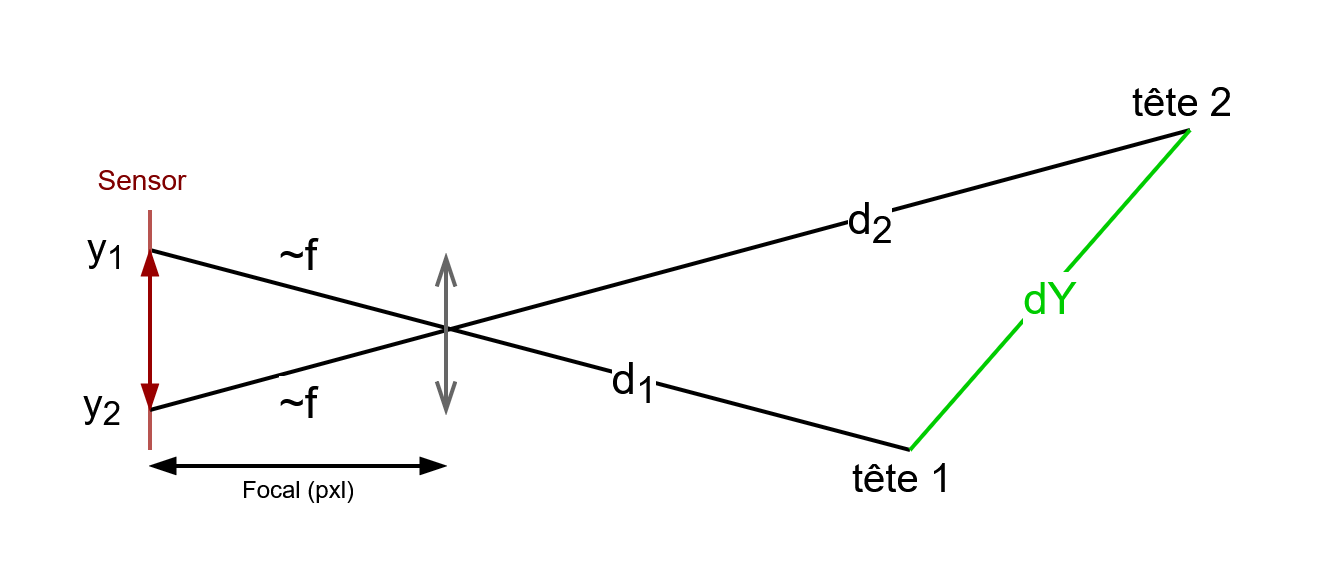
\includegraphics[width=0.45\textwidth]{images/dY_estimation.drawio.png}
    \caption{Modélisation pour la distance sur l'axe Y.}
    \label{fig:alkachy}
\end{figure}

\begin{equation}
    dY^2 = d_1^2 + d_2^2 - 2d_1d_2 ( 1 - ( \frac{|y_2-y_1|^2}{2*focal^2} ) )
\end{equation}

\subsection{distance sur l'axe X}

Pour la calculer la distance dans cette dimensions c'est assez facile, en utilisant la formume \ref{eq:camera-relation} on détermine la distance en mêtre au niveau de x1 avec d1, puis au niveau de x2 avec d2.
On fait l'hypothèse que la perspecive est parfaitement plongeante ce qui fait qu'il faut enlever la moitié de la différence pour obtenir la distance entre les 2 têtes (avec $d_2>d_1$).

\begin{align}
    dX1 &= (x_2-x_1) * d1 / focal \\
    dX2 &= (x_2-x_1) * d2 / focal \\
    dX  &= dX2 - (dX2-dX1)/2 \\
        &= (dX2 + dX1) /2
\end{align}

\subsection{distance totale}

Ainsi, on obtiens grâce au théorème de pythagore on peut calculer la distance inter-personnes en mètre.

\begin{figure}[h!]
    \centering
    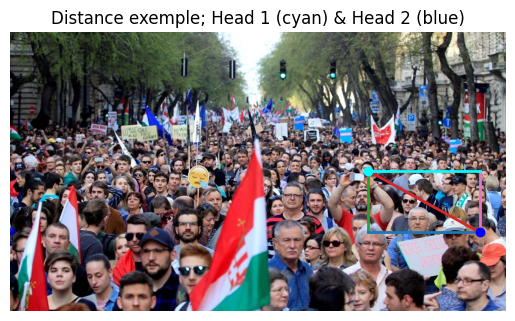
\includegraphics[width=0.45\textwidth]{images/exemple_dist_estimation.png}
    \caption{Exemple de distance estimé entre 2 têtes.}
    \label{fig:distance-estimation}
\end{figure}

Par exemple, sur notre exemple entre les 2 têtes de la Figure \ref{fig:distance-estimation}, on obtient les distances:

\begin{itemize}
    \item $d_1 = 20.82m (depth)$
    \item $d_2 = 10.9m (depth)$
    \item $dY = 9.93m$
    \item $dX = 1.12m$
    \item $d_{total} = 10.04m$
\end{itemize}

\section{Pour aller plus loin}

Grâce aux estimations de distances entre les têtes, on peut envisager plusieurs applications direct:

\begin{itemize}
    \item Soit construire un graphe de distance estimé entre les personnes dans le plan du sol.
    \item Soit placer directement les tête dans un espace 3D en utilisant les vecteurs de distance estimé, ce qui sera certainement plus précis 
\end{itemize}

Dans tous les cas ces mesures nous permettent d'estimer la densité de personnes dans une foule avec une simple caméra, et donc évaluer les risques associés ou simplement retracer les mouvements des personnes au cours du temps.

\section{Conclusion}

En conclusion, nous avons utilisé des modèles de deep learning avancés pour concevoir une application hybride efficace. Cette solution fusionne détection de têtes et estimation de profondeur, offrant des résultats satisfaisants.

Notre méthode présente des limites, notamment l’imprécision héritée des modèles combinés, qu’on a tenté de compenser. Une approche "end-to-end" aurait pu être plus précise, mais nous manquions du dataset nécessaire.

Ses atouts reposent sur l’utilisation de modèles pré-entraînés performants, demandant peu de ressources. Cela la rend idéale pour notre projet et facilement adaptable aux progrès futurs.

Enfin, il nous manque une évaluation chiffrée pour juger pleinement notre méthode. Une expérience réelle avec caméra ou une simulation via un moteur de jeu vidéo pourrait serait la prochaine étape pour valider nos performances.


    \printbibliography


\end{document}
